\subsection{Automation}

\begin{figure}[h!]
  \centering
  \begin{subfigure}{.45\textwidth}
      \centering
      \frame{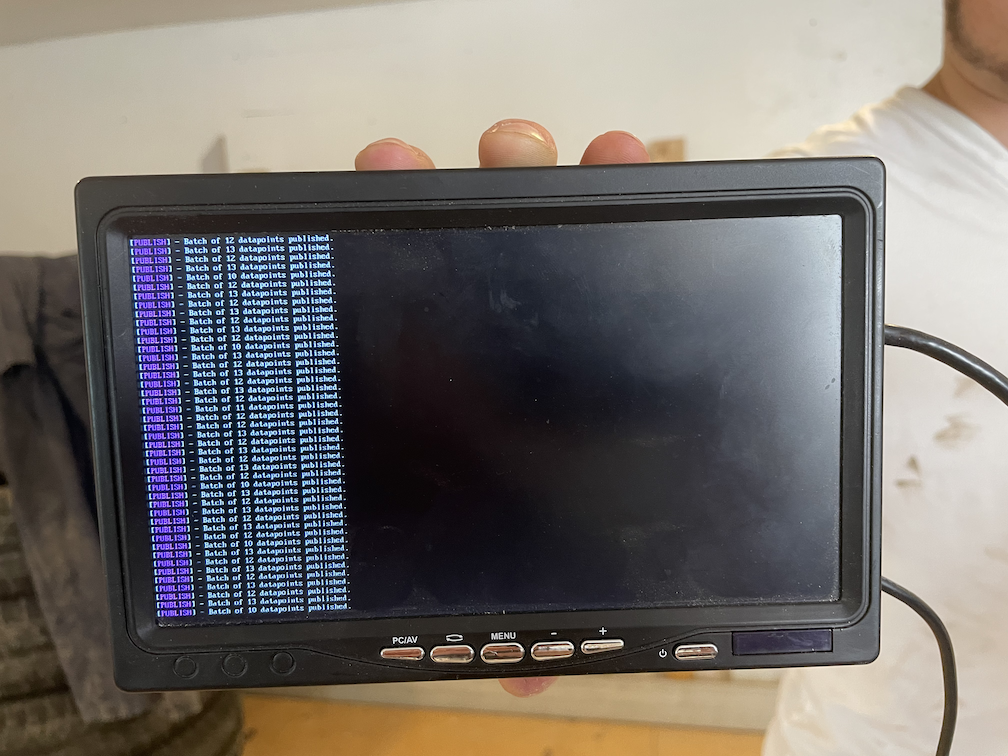
\includegraphics[width=\textwidth]{../assets/photos/prototype_automation_datapoints.png}}
      \caption{Automation example output. Datapoints collected from sensors are published in batches to minimize API calls.}
      \label{fig:prototype_automation_datapoints}
    \end{subfigure}
    \hspace{.05\textwidth}
    \begin{subfigure}{.45\textwidth}
      \centering
      \frame{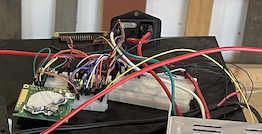
\includegraphics[width=\textwidth]{../assets/photos/prototype_automation_wiring.png}}
      \caption{Automation wiring on breadboard. Includes computer, microcontroller, CO2 sensor, temperature and humidity sensor, and lighting control signals.}
      \label{fig:prototype_automation_wiring}
    \end{subfigure}
    \caption{Automation prototype.}
\end{figure}

The prototype performs all functions as designed. All automation software can be found on our GitHub:\\ \href{https://github.com/PeaPodTechnologies/PeaPod/tree/staging/software}{https://github.com/PeaPodTechnologies/PeaPod/tree/staging/software}